\documentclass[12pt,a4paper]{article}

% =========================
% Font và ngôn ngữ tiếng Việt
% =========================
\usepackage{fontspec}
\usepackage{polyglossia}
\setmainlanguage{vietnamese}
\setmainfont{Times New Roman}

% =========================
% Hình ảnh và bảng
% =========================
\usepackage{graphicx}
\usepackage{longtable}
\usepackage{booktabs}
\usepackage{float}

% =========================
% Định dạng văn bản
% =========================
\usepackage{parskip}
\usepackage{setspace}
\usepackage{enumitem}

% =========================
% Hộp nội dung
% =========================
\usepackage[most]{tcolorbox}

% =========================
% TikZ
% =========================
\usepackage{tikz}
\usetikzlibrary{calc}
\usepackage{pgfornament}

% =========================
% Căn lề
% =========================
\usepackage[
    a4paper,
    top=2cm,
    bottom=2cm,
    left=2cm,
    right=2cm
]{geometry}

% =========================
% Liên kết và mục lục
% =========================
\usepackage[
    colorlinks=true,
    linkcolor=black,
    urlcolor=blue,
    citecolor=black
]{hyperref}

\usepackage{etoolbox}

\makeatletter
\renewcommand{\@seccntformat}[1]{%
  \ifstrequal{#1}{section}%
    {Chương~\csname the#1\endcsname:\ }%   % section: thêm "Chương"
    {\csname the#1\endcsname\quad}%        % các cấp khác: giữ mặc định
}
\makeatother

\usepackage{xltabular} % Kết hợp tính năng ngắt trang của longtable và chỉnh độ rộng của tabularx
\usepackage{array}

\setlength{\parindent}{2em}

\begin{document}

\begin{titlepage}
\begin{tikzpicture}[remember picture, overlay]

\draw[line width=2pt]
($(current page.north west)+(1cm,-1cm)$)
rectangle
($(current page.south east)+(-1cm,1cm)$);

\draw[line width=0.6pt]
($(current page.north west)+(1.3cm,-1.3cm)$)
rectangle
($(current page.south east)+(-1.3cm,1.3cm)$);

\end{tikzpicture}
\centering

% Header
{\bfseries TRƯỜNG ĐẠI HỌC GIAO THÔNG VẬN TẢI \\
KHOA CÔNG NGHỆ THÔNG TIN} \\[0.3cm]
---o0o--- \\[1cm]

% Logo

\includegraphics[width=0.3\textwidth]{images/utc_logo.png} \\[1cm]

% Title
{\Large \bfseries TÀI LIỆU ĐẶC TẢ PHẦN MỀM} \\[0.3cm]
{\bfseries HỌC PHẦN PROJECT 1} \\[0.5cm]

{\bfseries ĐỀ TÀI:} \\[0.3cm]
{\bfseries XÂY DỰNG WEBSITE QUẢN LÝ BÀI TẬP VÀ CHẤM CHỮA\\BÀI TIẾNG ANH THÔNG MINH  } \\[1.5cm]

% Info block
% \begin{center}
\setstretch{1.3}
% \hspace{4.5cm} % dịch toàn bộ khối sang phải thêm 1cm
\begin{minipage}{0.6\textwidth} % giảm độ rộng để khối nằm lệch phải hơn
\begin{flushleft}

\begin{center}
\begin{tabular}{p{5cm} p{8cm}}
\textbf{Giảng viên hướng dẫn:}
&
\textbf{TS. Nguyễn Trọng Phúc}
\\[0.2cm]

\textbf{Nhóm:}
&
\textbf{4}
\\[0.2cm]

\textbf{Sinh viên thực hiện:}
&
\textbf{Hồ Việt Tùng -- 231230949}
\\[0.2cm]

&
Đoàn Thái Sơn -- 231220886
\\[0.2cm]

&
Trần Tiến Sơn -- 231210892
\\[0.2cm]

&
Nguyễn Văn Tú -- 231230941
\\[0.2cm]

&
Phạm Minh Tuấn -- 231230946
\\
\end{tabular}
\end{center}

\end{flushleft}
\end{minipage}

\vfill

% Footer
{\centering Hà Nội, Tháng 4 Năm 2026}

\end{titlepage}

\begin{titlepage}
\centering

% Header
{\bfseries TRƯỜNG ĐẠI HỌC GIAO THÔNG VẬN TẢI \\
KHOA CÔNG NGHỆ THÔNG TIN} \\[0.3cm]
---o0o--- \\[1cm]

% Logo

\includegraphics[width=0.3\textwidth]{images/utc_logo.png} \\[1cm]

% Title
{\Large \bfseries TÀI LIỆU ĐẶC TẢ PHẦN MỀM} \\[0.3cm]
{\bfseries HỌC PHẦN PROJECT 1} \\[0.5cm]

{\bfseries ĐỀ TÀI:} \\[0.3cm]
{\bfseries XÂY DỰNG WEBSITE QUẢN LÝ BÀI TẬP VÀ CHẤM CHỮA\\BÀI TIẾNG ANH THÔNG MINH  } \\[1.5cm]

% Info block
% \begin{center}
\setstretch{1.3}
% \hspace{4.5cm} % dịch toàn bộ khối sang phải thêm 1cm
\begin{minipage}{0.6\textwidth} % giảm độ rộng để khối nằm lệch phải hơn
\begin{flushleft}

\begin{center}
\begin{tabular}{p{5cm} p{8cm}}
\textbf{Giảng viên hướng dẫn:}
&
\textbf{TS. Nguyễn Trọng Phúc}
\\[0.2cm]

\textbf{Nhóm:}
&
\textbf{4}
\\[0.2cm]

\textbf{Sinh viên thực hiện:}
&
\textbf{Hồ Việt Tùng -- 231230949}
\\[0.2cm]

&
Đoàn Thái Sơn -- 231220886
\\[0.2cm]

&
Trần Tiến Sơn -- 231210892
\\[0.2cm]

&
Nguyễn Văn Tú -- 231230941
\\[0.2cm]

&
Phạm Minh Tuấn -- 231230946
\\
\end{tabular}
\end{center}

\end{flushleft}
\end{minipage}

\vfill

% Footer
{\centering Hà Nội, Tháng 4 Năm 2026}

\end{titlepage}

% Lời cảm ơn
\begin{center}
    \section*{Lời cảm ơn}
\end{center}

Lời đầu tiên nhóm chúng em xin chân thành cảm ơn thầy Nguyễn Trọng Phúc đã nhiệt tình giảng dạy và truyền đạt cho chúng em những kiến thức quan trọng trong suốt học phần Project I. Những kiến thức và góp ý của thầy đã góp phần giúp nhóm hoàn thiện đề tài này. 

Do kiến thức chuyên môn còn hạn chế nên nhóm chúng em sẽ không tránh khỏi những thiếu sót trong bài, nhóm chúng em hi vọng sẽ nhận được thêm những góp ý của thầy để giúp đề tài hoàn thiện hơn. 

Chúng em xin chân thành cảm ơn thầy! 

\clearpage

\tableofcontents

\clearpage

\listoffigures

\clearpage

\listoftables

\clearpage

\begin{center}
\section*{Lời mở đầu}
\addcontentsline{toc}{section}{Lời mở đầu}
\end{center}

\setcounter{subsection}{0}

\subsection*{Tính cấp thiết của bài toán}

Trong bối cảnh toàn cầu hóa và hội nhập quốc tế sâu rộng, tiếng Anh đã trở thành một kỹ năng thiết yếu đối với học sinh, sinh viên cũng như người lao động. Nhu cầu học tập ngôn ngữ này ngày càng cấp thiết, dẫn đến sự phát triển mạnh mẽ của các trung tâm tiếng Anh. Số liệu từ Sở Giáo dục và Đào tạo TP.HCM cho thấy sự bùng nổ mạnh mẽ của các cơ sở đào tạo tiếng Anh, với 2.380 trung tâm hiện hành, cao gấp 6 lần so với con số 370 của năm 2010. Tương tự, Hà Nội cũng ghi nhận mức tăng trưởng gần gấp đôi trong 6 năm, từ 562 cơ sở (tháng 8/2018) lên 955 cơ sở vào cuối năm 2024 (VnExpress, 2025).

Tuy nhiên, sự gia tăng về số lượng học viên và sự đa dạng của các khóa học đã tạo ra nhiều thách thức trong công tác quản lý. Thực tế cho thấy, phương pháp quản lý thủ công bằng giấy tờ hoặc các tệp tin rời rạc không chỉ dễ gây thất lạc, sai sót thông tin mà còn làm tốn nhiều thời gian tra cứu. Bên cạnh đó, việc theo dõi tiến độ học tập và điểm số của từng học viên chưa được hệ thống hóa, gây khó khăn cho việc quản lý và phản hồi kịp thời cho phụ huynh. Tình trạng này còn thể hiện ở công tác quản lý học phí, khi các khoản thu chi chưa được đồng bộ, dẫn đến thiếu minh bạch và dễ phát sinh nhầm lẫn. Những yếu tố này khiến việc tổng hợp dữ liệu để lập báo cáo, thống kê trở nên nặng nề, đòi hỏi nhiều thời gian và nhân lực, làm giảm hiệu quả hoạt động chung của trung tâm.

Xuất phát từ thực tiễn đó, nhóm chúng em thực hiện bài tập lớn môn Phân tích thiết kế hướng đối tượng dưới sự hướng dẫn của Tiến sĩ Nguyễn Hiếu Cường, với đề tài: “Quản lý học viên trung tâm tiếng Anh”. Bài tập lớn này là cơ hội để nhóm tiếp cận và áp dụng phương pháp phát triển phần mềm theo hướng đối tượng, từ việc khảo sát yêu cầu, xây dựng mô hình phân tích đến thiết kế hệ thống. Thông qua đó, nhóm tiến hành mô hình hóa hệ thống bằng các kỹ thuật tiêu biểu như Use Case, Domain Model, Sequence Diagram và Design Class Diagram nhằm đảm bảo hệ thống được thiết kế một cách chặt chẽ, rõ ràng và có khả năng mở rộng.

Mục tiêu của đề tài là xây dựng một bản thiết kế hệ thống quản lý học viên tại trung tâm tiếng Anh dựa trên phương pháp hướng đối tượng, đảm bảo tính đầy đủ về chức năng, hợp lý về mặt kiến trúc và rõ ràng trong mô hình tương tác giữa các đối tượng. Qua quá trình thực hiện, nhóm mong muốn nâng cao khả năng phân tích, tư duy thiết kế hệ thống và tích lũy kinh nghiệm thực tiễn trong việc phát triển phần mềm theo chuẩn công nghiệp.

Để thực hiện mục tiêu trên, nhóm đã tiến hành thu thập yêu cầu của khách hàng tại một số trung tâm tiếng Anh thông qua phỏng vấn trực tiếp và sử dụng phiếu khảo sát. Sau đó, nhóm xây dựng tài liệu đặc tả yêu cầu phần mềm (SRS), xác định các yêu cầu chức năng và phi chức năng, và tiến hành mô hình hóa hệ thống theo hướng đối tượng. Các mô hình được xây dựng bao gồm Use Case Diagram, Use Case Specification, Domain Model, CRC Cards, BCE Architecture, Sequence Diagram và các biểu đồ thiết kế chi tiết nhằm mô tả đầy đủ cấu trúc và hành vi của hệ thống.

\clearpage

\begin{center}
\section*{Bảng phân công nhiệm vụ}
\addcontentsline{toc}{section}{Bảng phân công nhiệm vụ}
\end{center}

\begin{xltabular}{\textwidth}{|p{3cm}|p{3cm}|X|}
% --- Tiêu đề và Đầu bảng ở TRANG ĐẦU TIÊN ---
\hline
\multicolumn{1}{|c|}{\textbf{Vị trí}} & \multicolumn{1}{c|}{\textbf{Tên thành viên}} & \multicolumn{1}{c|}{\textbf{Nhiệm vụ}} \\ \hline
\endfirsthead
\hline
\endlastfoot

Project Manager (PM) & Hồ Việt Tùng & Xây dựng kế hoạch tổng thể và theo dõi tiến độ triển khai của dự án. Chủ động nhìn nhận và xử lý các rào cản phát sinh trong quá trình thực hiện. Giám sát và đảm bảo chất lượng đầu ra của dự án.
\\ \hline

DevOps & Phạm Minh Tuấn, Hồ Việt Tùng & Thiết lập và quản trị hạ tầng phục vụ triển khai hệ thống. Xây dựng quy trình tích hợp và triển khai liên tục (CI/CD) nhằm tự động hóa quá trình deploy. Giám sát hiệu năng hệ thống, quản lý bảo mật và đảm bảo ứng dụng vận hành ổn định. 
\\ \hline

Frontend Developer & Trần Tiến Sơn & Xây dựng giao diện người dùng dựa trên bản thiết kế đã thống nhất. Tích hợp API từ Backend, xử lý logic hiển thị dữ liệu và đảm bảo ứng dụng hoạt động mượt mà, tương thích tốt trên nhiều loại thiết bị và trình duyệt. 
\\ \hline

Backend Developer & Đoàn Thái Sơn, Phạm Minh Tuấn & Thiết kế kiến trúc cơ sở dữ liệu và phát triển các API RESTful. Xử lý các logic nghiệp vụ cốt lõi, quản lý xác thực/phân quyền người dùng và tối ưu hóa hiệu suất xử lý dữ liệu phía server nhằm đảm bảo tốc độ phản hồi.
\\ \hline

Tester & Nguyễn Văn Tú & Phân tích yêu cầu và xây dựng test case phù hợp cho từng chức năng. Thực hiện kiểm thử phần mềm bằng phương pháp thủ công hoặc tự động nhằm phát hiện các lỗi về chức năng, giao diện và hiệu năng. Phối hợp với nhóm Dev để tái hiện và khắc phục lỗi trước khi phát hành. 
\\ \hline

\end{xltabular}

\clearpage

\begin{center}
\section{Giới thiệu}
\end{center}

\subsection{Mục đích}

Mục tiêu của dự án là xây dựng một website quản lý bài tập và chấm chữa bài tiếng Anh, tập trung vào việc hỗ trợ giáo viên giao bài, mở/khóa bài tập, chấm điểm và chữa bài (kết hợp chấm chữa thông minh bằng AI) cho học viên trên cả 4 kỹ năng Nghe – Nói – Đọc – Viết theo từng lớp học; đồng thời cho phép học viên làm bài, nộp bài, xem lại phần chữa bài và theo dõi kết quả trực tuyến. Hệ thống có tích hợp chức năng quản lý cơ bản về học viên, lớp học, điểm số, và một phân hệ Admin dành cho trung tâm để quản lý tài khoản người dùng. 

\subsection{Phạm vi}

Đối tượng sử dụng website là quản lý trung tâm, giáo viên, học viên.

\subsection{Thuật ngữ/ từ viết tắt}

\subsection{Tài liệu tham khảo}

\clearpage

\begin{center}
\section{Công cụ và công nghệ sử dụng}
\end{center}

\subsection{Công nghệ}

\begin{itemize}
  \item \textbf{Backend:} Java, Spring Boot, Spring Data JPA + Hibernate, Flyway
  \item \textbf{Frontend:} ReactJS, Vite, TypeScript, Shadcn, Ant Design, Tailwind
  \item \textbf{Database:} PostgreSQL
\end{itemize}

\subsection{Công cụ}

\begin{itemize}
  \item \textbf{Quản lý dự án và phân công nhiệm vụ:} Trello
  \item \textbf{Quản lý bug:} Excel
  \item \textbf{Giao tiếp đội nhóm:} Messenger, Discord
  \item \textbf{Kiểm thử giao diện thủ công:} Chrome DevTools
  \item \textbf{IDE:} Visual Studio Code, IntelliJ IDEA
  \item \textbf{Quản lý tài liệu dự án:} OneDrive, Google Drive
  \item \textbf{Quản lý mã nguồn:} GitHub
  \item \textbf{Kiểm thử API:} Postman
  \item \textbf{Công cụ đóng gói:} Docker
  \item \textbf{Thiết kế UI:} Balsamiq, Figma
  \item \textbf{Vẽ biểu đồ:} Draw.io, Excalidraw, Mermaid
  \item \textbf{SQL client:} pgAdmin 4, PostgreSQL, DBeaver
  \item \textbf{Kiểm thử tự động:} Selenium, TestNG
\end{itemize}

\clearpage

\begin{center}
\section{Yêu cầu chức năng}
\end{center}

\subsection{Tác nhân}

Hệ thống gồm có các tác nhân là Học viên, Giáo viên và Quản trị viên. Quản trị viên có vai trò quản trị hoạt động của hệ thống, giáo viên có vai trò quản lý lớp học, quản lý học viên trong lớp học, quản lý bài tập của học viên, quản lý bài tập.

\subsection{Xác định các ca sử dụng}

\begin{xltabular}{\textwidth}{|c|p{3.5cm}|X|p{3.5cm}|}
% --- Tiêu đề và Đầu bảng ở TRANG ĐẦU TIÊN ---
\caption{Danh sách Ca sử dụng (Use Cases)} \label{tab:use_cases} \\
\hline
\multicolumn{1}{|c|}{\textbf{STT}} & \multicolumn{1}{|c|}{\textbf{Ca sử dụng}} & \multicolumn{1}{|c|}{\textbf{Mô tả ngắn}} & \multicolumn{1}{|c|}{\textbf{Tác nhân}} \\ \hline
\endfirsthead
\hline
\endlastfoot

% --- DỮ LIỆU BẢNG ---
1 & Đăng nhập & Người dùng đăng nhập vào hệ thống bằng tài khoản và mật khẩu. & Quản lý, Giáo viên, Học viên \\ \hline
2 & Đăng xuất & Người dùng đăng xuất khỏi tài khoản đang sử dụng. & Quản lý, Giáo viên, Học viên \\ \hline
3 & Quản lý tài khoản cá nhân & Người dùng xem và cập nhật thông tin cá nhân, mật khẩu và các thông tin liên quan. & Quản lý, Giáo viên, Học viên \\ \hline
4 & Quản lý tài khoản người dùng & Quản lý trung tâm tạo, cập nhật, khóa/mở khóa và quản lý tài khoản người dùng. & Quản lý \\ \hline
5 & Phân quyền người dùng & Quản lý trung tâm thiết lập và quản lý quyền truy cập theo vai trò của người dùng. & Quản lý \\ \hline
6 & Quản lý giáo viên & Quản lý trung tâm xem, thêm, cập nhật và quản lý thông tin giáo viên. & Quản lý \\ \hline
7 & Quản lý học viên & Quản lý trung tâm quản lý thông tin, tài khoản và trạng thái của học viên. & Quản lý \\ \hline
8 & Quản lý lớp học & Quản lý trung tâm tạo, cập nhật, xem và quản lý lớp học, cập nhật giáo viên quản lý lớp. & Quản lý \\ \hline
9 & Quản lý thành viên lớp học & Quản lý trung tâm hoặc giáo viên thêm, xóa và quản lý học viên thuộc lớp học. & Quản lý, Giáo viên \\ \hline
10 & Xem danh sách lớp học & Người dùng xem các lớp học mà mình được tham gia hoặc quản lý. & Giáo viên, Học viên \\ \hline
11 & Quản lý bài tập & Giáo viên tạo, chỉnh sửa, xóa, xem và quản lý các bài tập theo lớp học. & Giáo viên \\ \hline
12 & Tạo bài tập & Giáo viên tạo bài tập, thiết lập nội dung, thời gian, điểm số và các yêu cầu làm bài. & Giáo viên \\ \hline
13 & Mở bài tập & Giáo viên mở bài tập để học viên có thể truy cập và thực hiện. & Giáo viên \\ \hline
14 & Khóa bài tập & Giáo viên khóa bài tập để ngăn học viên tiếp tục làm hoặc nộp bài. & Giáo viên \\ \hline
15 & Xem bài tập & Học viên xem danh sách, nội dung, thời hạn và trạng thái của các bài tập được giao. & Học viên \\ \hline
16 & Làm bài tập viết & Học viên thực hiện và nộp bài tập kỹ năng Viết. & Học viên \\ \hline
17 & Làm bài tập nói & Học viên thực hiện bài tập Nói, ghi âm hoặc tải lên phần trả lời và nộp bài. & Học viên \\ \hline
18 & Làm bài tập đọc & Học viên thực hiện các câu hỏi và bài tập kỹ năng Đọc. & Học viên \\ \hline
19 & Làm bài tập nghe & Học viên nghe nội dung và thực hiện các câu hỏi của bài tập Nghe. & Học viên \\ \hline
20 & Nộp bài tập & Học viên hoàn thành và gửi bài làm lên hệ thống để chấm điểm. & Học viên \\ \hline
21 & Xem trạng thái bài làm & Học viên theo dõi trạng thái bài làm như chưa làm, đã nộp, đã chấm hoặc đã chữa. & Học viên \\ \hline
22 & Chấm bài & Giáo viên xem bài làm và thực hiện chấm điểm cho học viên. & Giáo viên \\ \hline
23 & Hỗ trợ chấm chữa bài bằng AI & Hệ thống sử dụng AI để phân tích bài làm, đưa ra điểm số, nhận xét và gợi ý sửa lỗi. & Giáo viên \\ \hline
24 & Hỗ trợ chấm chữa bài viết bằng AI & AI phân tích bài viết, phát hiện lỗi ngữ pháp, từ vựng, chính tả, diễn đạt và đưa ra nhận xét. & Giáo viên \\ \hline
25 & Hỗ trợ chấm chữa bài nói bằng AI & AI phân tích phần nói dựa trên nội dung và các tiêu chí phù hợp như phát âm, từ vựng, ngữ pháp và độ trôi chảy. & Giáo viên \\ \hline
26 & Chấm bài đọc & Hệ thống tự động chấm các câu trả lời của bài Đọc và tính điểm. & Giáo viên \\ \hline
27 & Chấm bài nghe & Hệ thống tự động chấm các câu trả lời của bài Nghe và tính điểm. & Giáo viên \\ \hline
28 & Xem điểm số & Người dùng xem điểm của các bài tập và kết quả học tập. & Giáo viên, Học viên \\ \hline
29 & Xem kết quả học tập & Học viên theo dõi kết quả và tiến độ học tập theo bài tập, kỹ năng hoặc lớp học. & Học viên \\ \hline
30 & Xem bài chữa & Học viên xem nhận xét, lỗi sai, đáp án và hướng dẫn sửa bài sau khi được chấm. & Học viên \\ \hline
31 & Xem và đánh giá kết quả học viên & Giáo viên xem điểm số, bài làm và kết quả học tập của học viên trong lớp. & Giáo viên \\ \hline
32 & Quản lý điểm số & Giáo viên xem, cập nhật và quản lý điểm số của học viên trong lớp. & Giáo viên \\ \hline
33 & Theo dõi tiến độ học tập & Giáo viên theo dõi tình trạng làm bài và kết quả của học viên theo từng kỹ năng. & Giáo viên \\

\end{xltabular}

\clearpage

\subsection{Sơ đồ ca sử dụng}

\begin{figure}[H]
    \centering
    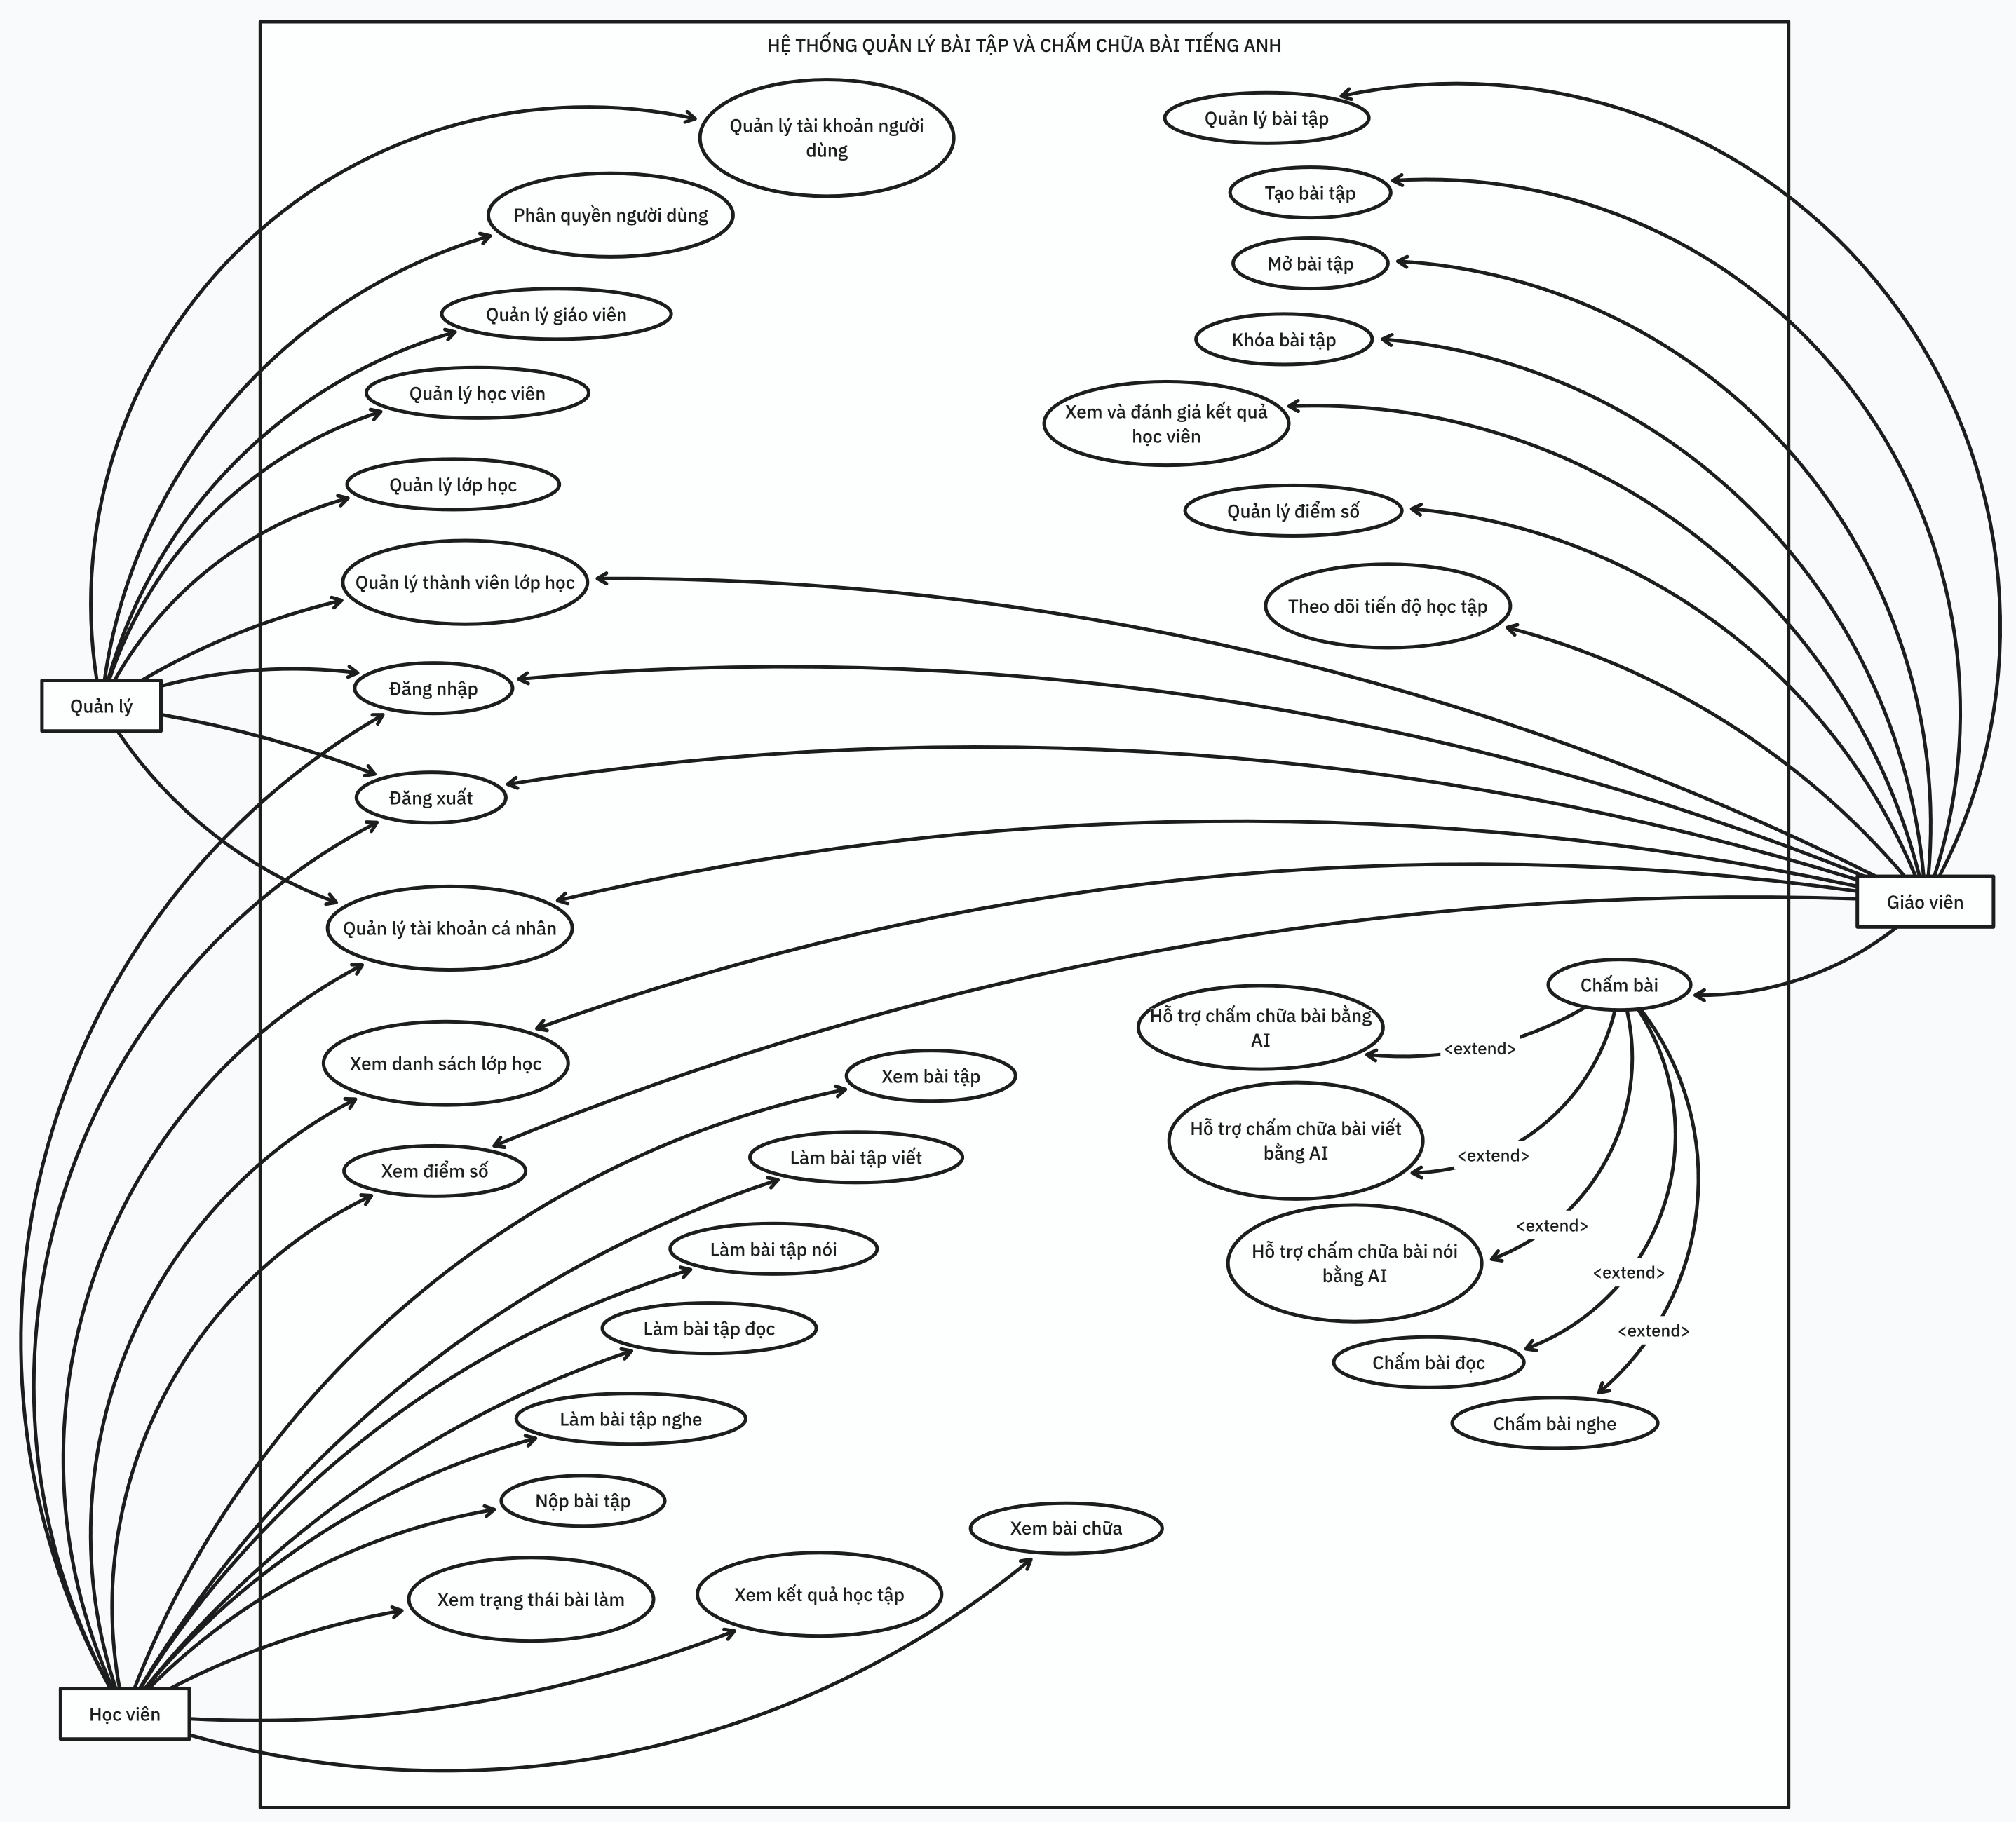
\includegraphics[width=0.85\textwidth]{images/Usecase/Usecase Diagram - Image.png}
    \caption{Sơ đồ ca sử dụng tổng quan}
    \label{fig:demo}
\end{figure}

\subsection{Biểu đồ hoạt động, đặc tả use case và UI}

\clearpage

\begin{center}
\section{Yêu cầu phi chức năng}
\end{center}

\clearpage

\end{document}